\documentclass[border=10pt]{standalone}
\usepackage[svgnames]{xcolor}
\usepackage{amsmath}
\usepackage{pgfplots}
\pgfplotsset{compat=newest}
\usepackage[sfdefault]{FiraSans}
\usepackage{FiraMono}
\renewcommand*\familydefault{\sfdefault}
\begin{document}
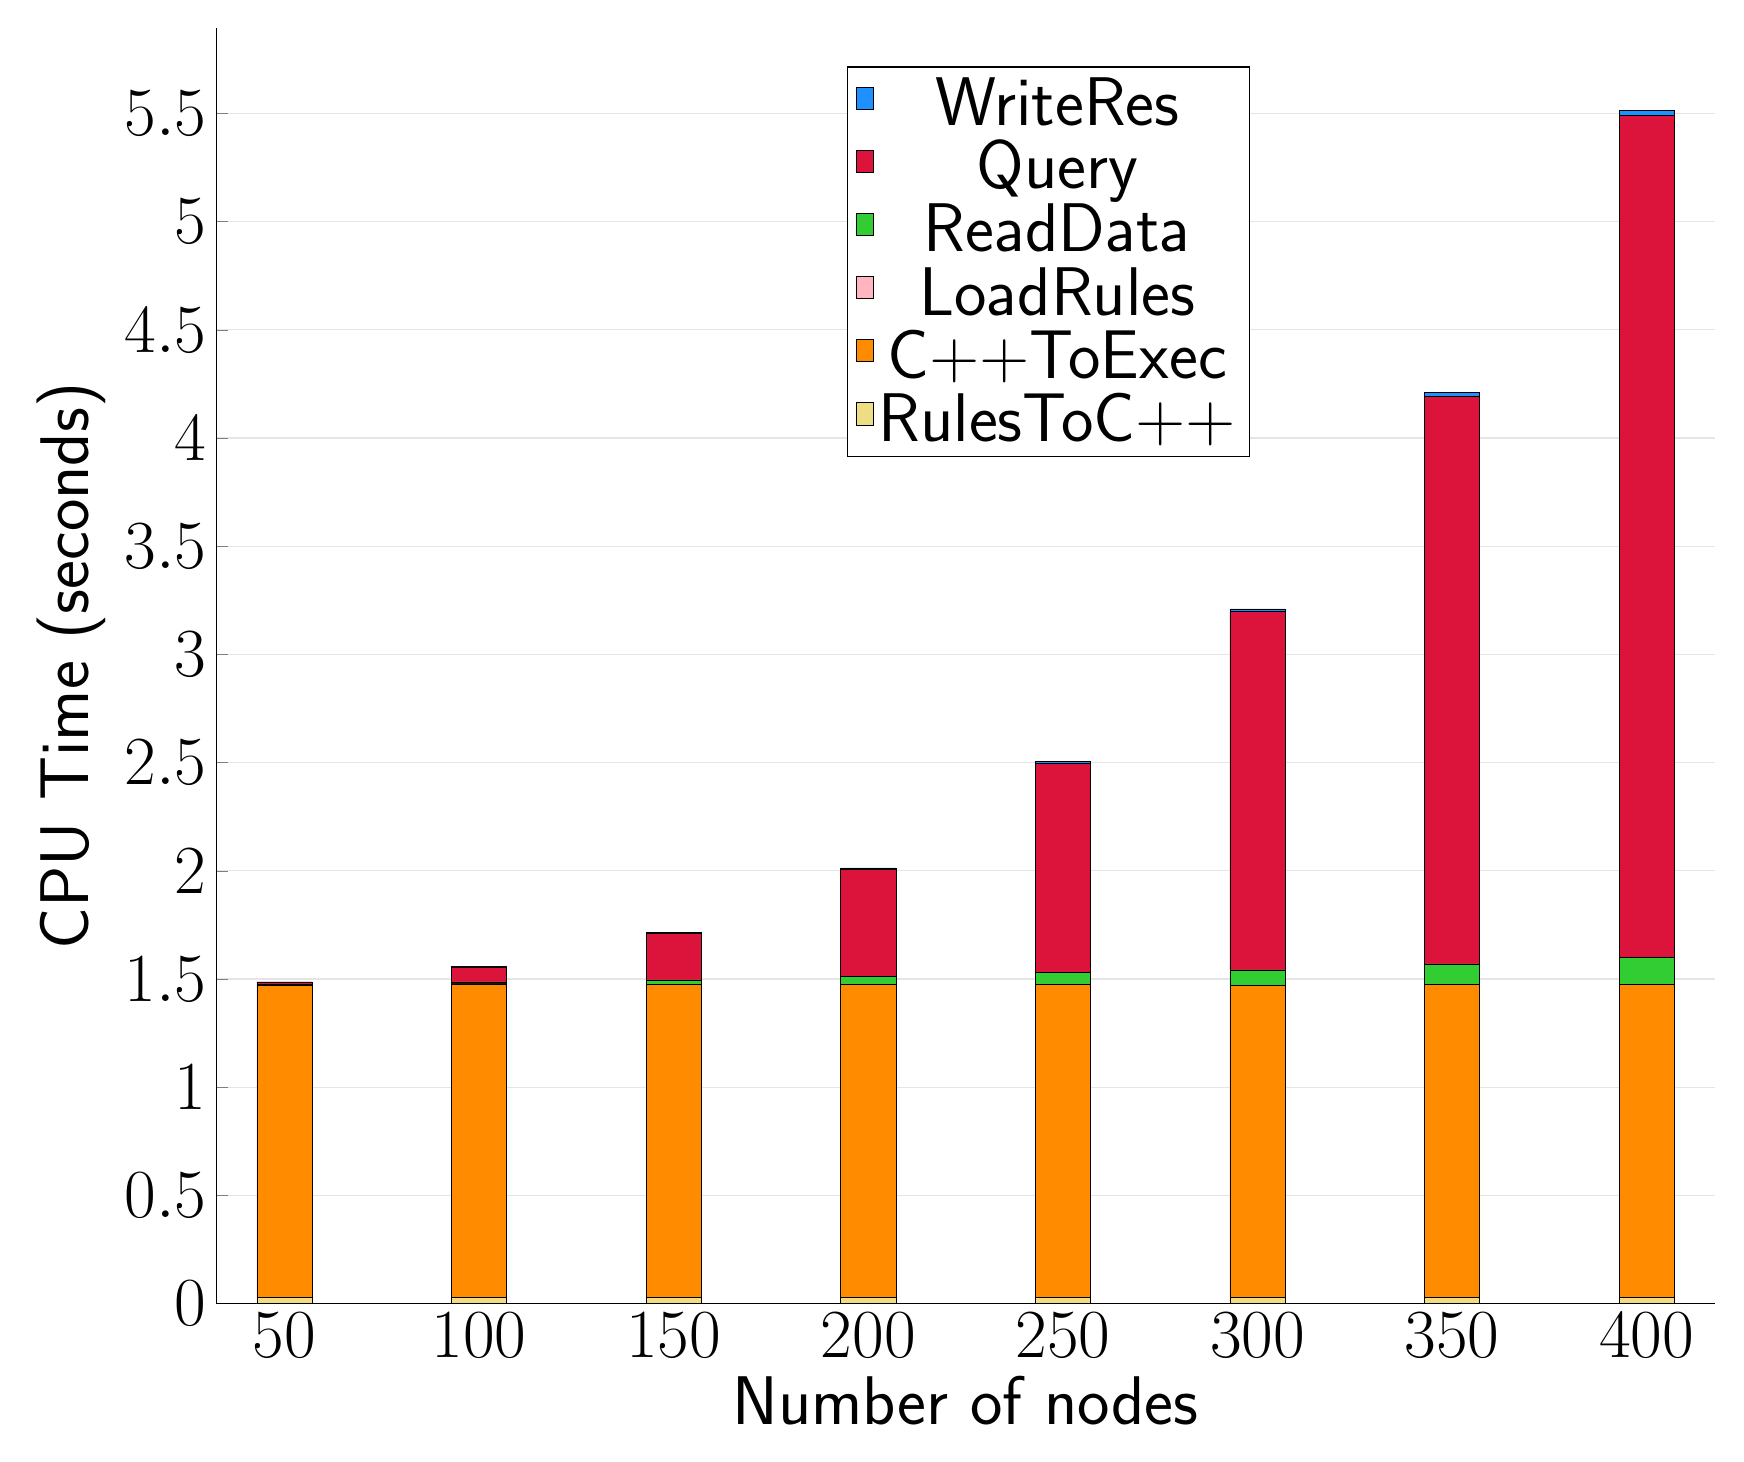
\begin{tikzpicture}
\begin{axis}[
   ybar stacked,
   width=1.7\textwidth,
   bar width=0.7cm,
   ymajorgrids, tick align=inside,
   major grid style={draw=gray!20},
   xtick=data,
   ymin=0, ymax=5.893940000000001,
   axis x line*=bottom,
   axis y line*=left,
   enlarge x limits=0.05,
   legend style={
       at={(0.69, 0.97)},
       anchor=north east,
       legend columns=1,
       font=\Huge,
   },
   ylabel={CPU Time (seconds)},
   xlabel={Number of nodes},
   label style={font=\Huge},
   tick label style={font=\Huge},
]
\addlegendimage{fill=DodgerBlue, draw=black, line width=0.2pt}
\addlegendentry{WriteRes}
\addlegendimage{fill=Crimson, draw=black, line width=0.2pt}
\addlegendentry{Query}
\addlegendimage{fill=LimeGreen, draw=black, line width=0.2pt}
\addlegendentry{ReadData}
\addlegendimage{fill=LightPink, draw=black, line width=0.2pt}
\addlegendentry{LoadRules}
\addlegendimage{fill=DarkOrange, draw=black, line width=0.2pt}
\addlegendentry{C++ToExec}
\addlegendimage{fill=LightGoldenrod, draw=black, line width=0.2pt}
\addlegendentry{RulesToC++}
\addplot +[fill=LightGoldenrod, draw=black, line width=0.2pt] coordinates {
(50, 0.030000000000000006)
(100, 0.030000000000000006)
(150, 0.030000000000000006)
(200, 0.030000000000000006)
(250, 0.030000000000000006)
(300, 0.030000000000000006)
(350, 0.030000000000000006)
(400, 0.030000000000000006)
};
\addplot +[fill=DarkOrange, draw=black, line width=0.2pt] coordinates {
(50, 1.4409999999999996)
(100, 1.448)
(150, 1.444)
(200, 1.4439999999999997)
(250, 1.4459999999999997)
(300, 1.4409999999999998)
(350, 1.4439999999999995)
(400, 1.4449999999999996)
};
\addplot +[fill=LightPink, draw=black, line width=0.2pt] coordinates {
(50, 0.0001197)
(100, 6.23e-05)
(150, 0.000125)
(200, 0.00012030000000000001)
(250, 0.00012169999999999998)
(300, 9.620000000000001e-05)
(350, 0.00010890000000000002)
(400, 0.0001275)
};
\addplot +[fill=LimeGreen, draw=black, line width=0.2pt] coordinates {
(50, 0.0028233)
(100, 0.0088252)
(150, 0.022247499999999996)
(200, 0.037603399999999995)
(250, 0.0546508)
(300, 0.07162400000000001)
(350, 0.09626309999999999)
(400, 0.12342810000000001)
};
\addplot +[fill=Crimson, draw=black, line width=0.2pt] coordinates {
(50, 0.0126552)
(100, 0.06914200000000001)
(150, 0.21575950000000002)
(200, 0.4960197)
(250, 0.9646997)
(300, 1.6551380000000002)
(350, 2.623153)
(400, 3.8939400000000006)
};
\addplot +[fill=DodgerBlue, draw=black, line width=0.2pt] coordinates {
(50, 0.000651)
(100, 0.0014976999999999998)
(150, 0.0032937)
(200, 0.0056438)
(250, 0.008795500000000001)
(300, 0.012630800000000001)
(350, 0.0170334)
(400, 0.0221109)
};
\end{axis}
\end{tikzpicture}

\end{document}
